%\documentclass[aspectratio=43]{beamer}

%
\documentclass[10pt]{beamer}

\usepackage{xeCJK}
\setCJKmainfont{蘋方-繁}

\setbeamertemplate{caption}[numbered] %加入圖片

\usetheme[progressbar=frametitle]{metropolis}
\usepackage{appendixnumberbeamer}
\usepackage{color}

\usepackage{booktabs}
\usepackage[scale=2]{ccicons}

\usepackage{pgfplots}
\usepgfplotslibrary{dateplot}

\usepackage{xspace}
\usepackage{listings}
\newcommand{\themename}{\textbf{\textsc{metropolis}}\xspace}
%

%\usepackage[english]{babel}
%\usepackage{mathtools}
%\usepackage{amsmath}

%\usepackage[backend=biber]{biblatex}

%\usepackage{amsthm}
\usepackage{mathtools}
\usepackage{physics}
\usepackage{calligra}
\usepackage{csquotes}
\usepackage{tensor}
\usepackage[thicklines]{cancel}
\usepackage{tcolorbox}
\usepackage{pstricks}
\usepackage[backend=biber, bibstyle=nature, sorting=nty, citestyle=numeric-comp]{biblatex} %Custom bibliography
    \addbibresource{bib.bib} %Load references


\DeclareMathAlphabet{\mathcalligra}{T1}{calligra}{m}{n}
\DeclareFontShape{T1}{calligra}{m}{n}{<->s*[2.2]callig15}{}
\newcommand{\scriptr}{\mathcalligra{r}\,}
\newcommand{\boldscriptr}{\pmb{\mathcalligra{r}}\,}
\def\rc{\scriptr}
\def\brc{\boldscriptr}
\def\hrc{\hat\brc}
\newcommand{\ie}{\emph{i.e.}} %id est
\newcommand{\eg}{\emph{e.g.}} %exempli gratia
\newcommand{\rtd}[1]{\ensuremath{\left\lfloor #1 \right\rfloor}}
\newcommand{\dirac}[1]{\ensuremath{\delta \left( #1 \right)}}
\newcommand{\diract}[1]{\ensuremath{\delta^3 \left( #1 \right)}}
\newcommand{\e}{\ensuremath{\epsilon_0}}
\newcommand{\m}{\ensuremath{\mu_0}}
\newcommand{\V}{\ensuremath{\mathcal{V}}}
\newcommand{\prnt}[1]{\ensuremath{\left(#1\right)}} %parentheses
\newcommand{\colch}[1]{\ensuremath{\left[#1\right]}} %square brackets
\newcommand{\chave}[1]{\ensuremath{\left\{#1\right\}}}  %curly brackets

\useoutertheme{infolines}
\useinnertheme{rectangles}
\usefonttheme{professionalfonts}


\definecolor{orange}{HTML}{f28165}
\definecolor{gray}{HTML}{303030}
\definecolor{yellow}{HTML}{f0be52}
\definecolor{lightorange}{HTML}{f19e58}

\renewcommand{\CancelColor}{\color{orange}}

\makeatletter
\newcommand{\mybox}[1]{%
  \setbox0=\hbox{#1}%
  \setlength{\@tempdima}{\dimexpr\wd0+13pt}%
  \begin{tcolorbox}[colback=orange,colframe=orange,boxrule=0.5pt,arc=4pt,
      left=6pt,right=6pt,top=6pt,bottom=6pt,boxsep=0pt,width=\@tempdima]
    \textcolor{white}{#1}
  \end{tcolorbox}
}
\makeatother

\usecolortheme[named=orange]{structure}
\usecolortheme{sidebartab}
\usecolortheme{orchid}
\usecolortheme{whale}
\setbeamercolor{alerted text}{fg=yellow}
\setbeamercolor{block title alerted}{bg=alerted text.fg!90!black}
\setbeamercolor{block title example}{bg=lightorange!60!black}
\setbeamercolor{background canvas}{bg=gray}
\setbeamercolor{normal text}{bg=gray,fg=white}

\setbeamertemplate{footline}
        {
      \leavevmode%
      \hbox{%
      \begin{beamercolorbox}[wd=.333333\paperwidth,ht=2.25ex,dp=1ex,center]{author in head/foot}%
        \usebeamerfont{author in head/foot}\insertshortauthor~~(\insertshortinstitute)
      \end{beamercolorbox}%
      \begin{beamercolorbox}[wd=.333333\paperwidth,ht=2.25ex,dp=1ex,center]{title in head/foot}%
        \usebeamerfont{title in head/foot}\insertshorttitle
      \end{beamercolorbox}%
      \begin{beamercolorbox}[wd=.333333\paperwidth,ht=2.25ex,dp=1ex,center]{date in head/foot}%
        \usebeamerfont{date in head/foot}\insertshortdate{}%\hspace*{2em}

    %#turning the next line into a comment, erases the frame numbers
        %\insertframenumber{} / \inserttotalframenumber\hspace*{2ex} 

      \end{beamercolorbox}}%
      \vskip0pt%
    }


\setbeamertemplate{blocks}[rectangle]
\setbeamercovered{dynamic}

\setbeamertemplate{section page}
{
	\begin{centering}
		\begin{beamercolorbox}[sep=27pt,center]{part title}
			\usebeamerfont{section title}\insertsection\par
			\usebeamerfont{subsection title}\insertsubsection\par
		\end{beamercolorbox}
	\end{centering}
}

%\setbeamertemplate{subsection page}
%{
%	\begin{centering}
%		\begin{beamercolorbox}[sep=12pt,center]{part title}
%			\usebeamerfont{subsection title}\insertsubsection\par
%		\end{beamercolorbox}
%	\end{centering}
%}

\newcommand{\hlight}[1]{\colorbox{violet!50}{#1}}
\newcommand{\hlighta}[1]{\colorbox{red!50}{#1}}
\title{計量經濟學電腦實習課} %->->->->-> Check hyperref title <-<-<-<-<-
\subtitle{L4 IV, Qusi-Experiments}
\author[Boyie]{陳柏瑜 Chen Boyie}
\institute[NTU]{
    Graduate Institute of Economics\\
    National Taiwan University\\
    r08323004@ntu.edu.tw%
} %You can change the Institution if you are from somewhere else
\date{\today}
%\logo{\includegraphics[width= 0.2\textwidth]{images/a-logo.png}}

\begin{document}
    
    \frame{\titlepage}
    
    \begin{frame}{Brief}
        \tableofcontents
    \end{frame}
    
    \section{Instrument Variable EE12.2}
    %\frame{\sectionpage}

%%
\begin{frame}[fragile]{EE12.2}

我們直接從課本的Empirical Exercise 12.2來複習如何用Stata處理內生性問題,並實作2SLS。

\end{frame}

%%
\begin{frame}[fragile]{EE12.2 Questions}
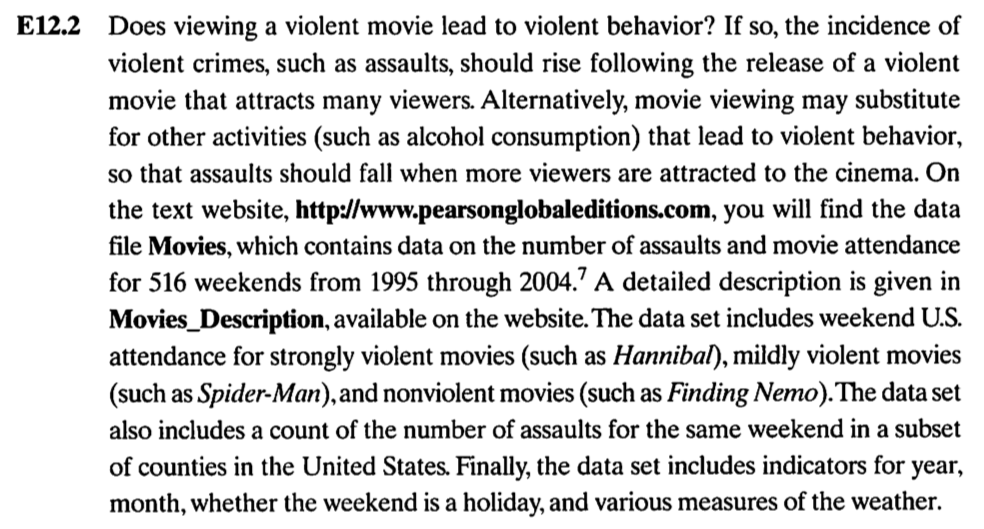
\includegraphics[width=1\textwidth]{Images/EE12-2_1.png}
\end{frame}
%%
\begin{frame}[fragile]{EE12.2 Questions}
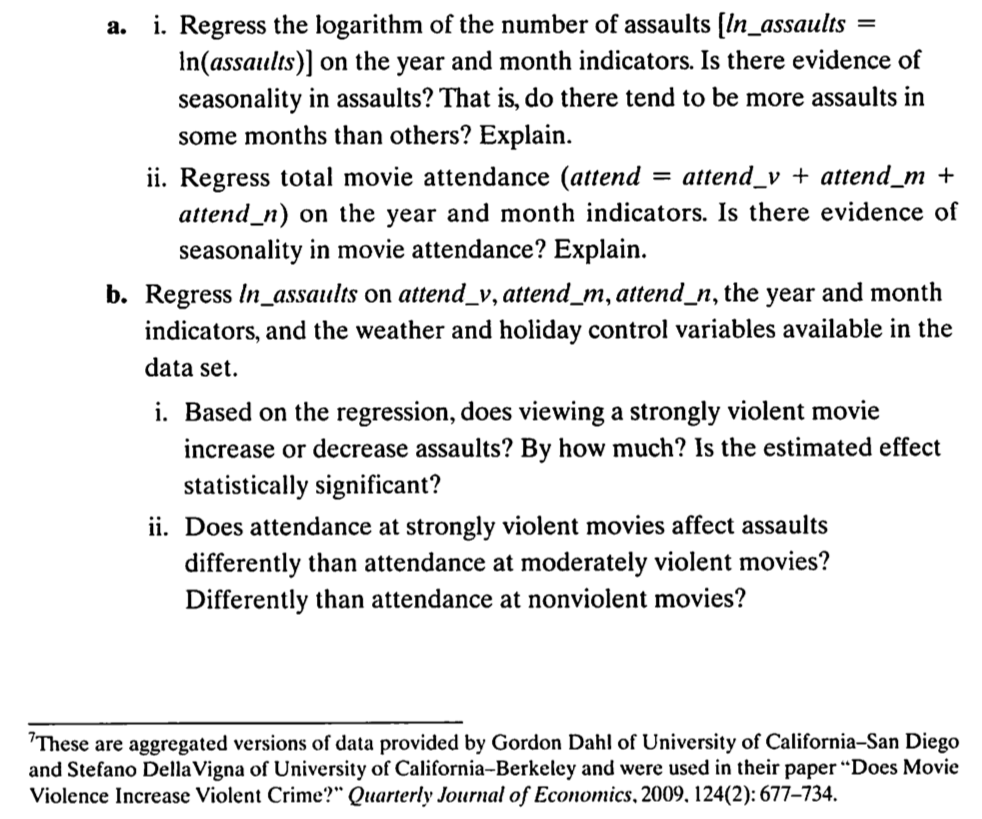
\includegraphics[width=1\textwidth]{Images/EE12-2_2.png}
\end{frame}
%%
\begin{frame}[fragile]{EE12.2 Questions}
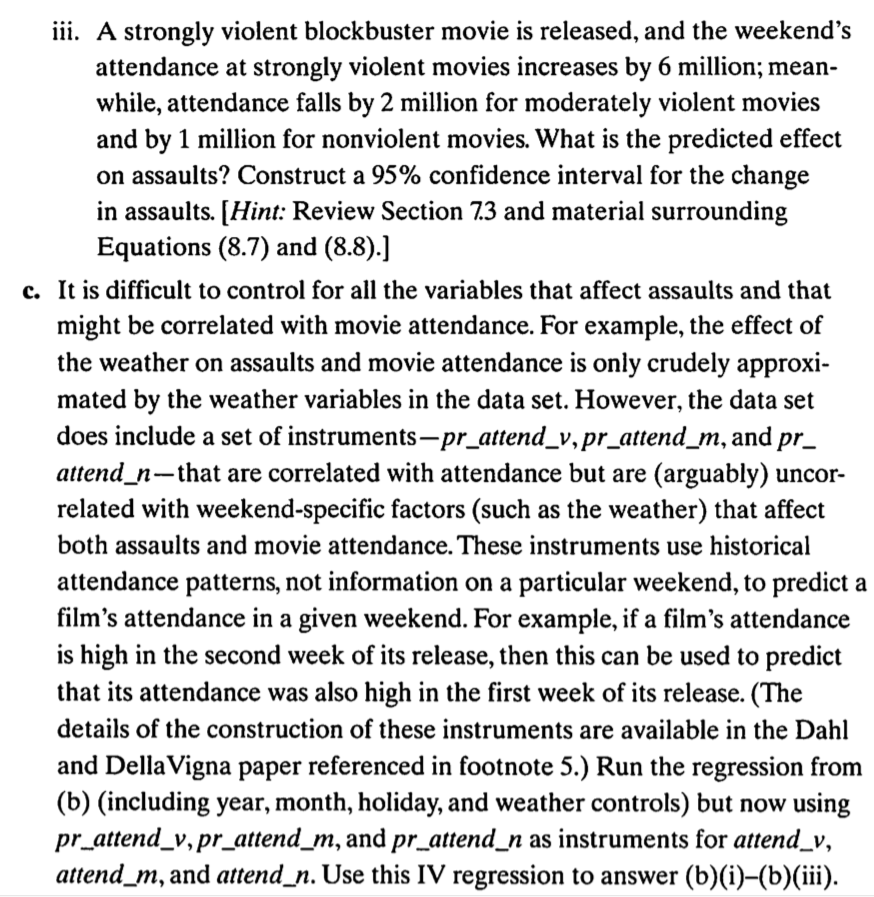
\includegraphics[width=0.6\textwidth]{Images/EE12-2_3.png}
\end{frame}
%%
\begin{frame}[fragile]{EE12.2 Questions}
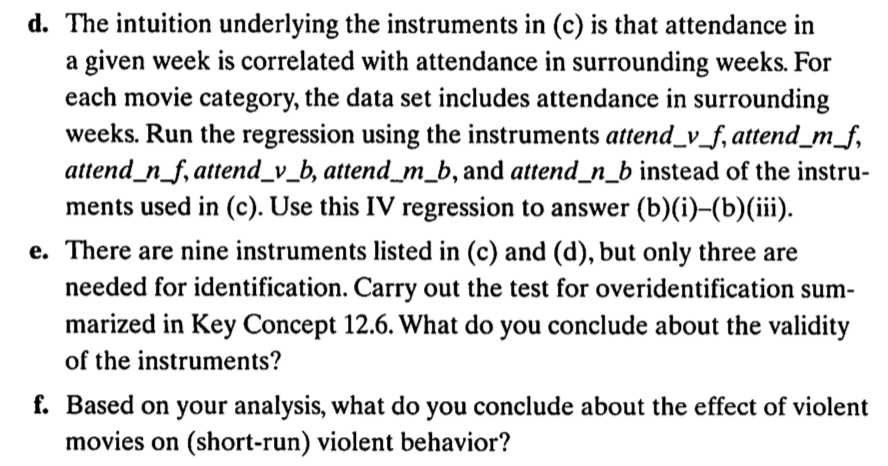
\includegraphics[width=1\textwidth]{Images/EE12-2_4.png}
\end{frame}


%%
\begin{frame}[fragile]{EE12.2 Data Descrptions}

Movie Data

\begin{enumerate}
    \item Observations: 516 weekends
    \item Time Period : 1995-2004
\end{enumerate}
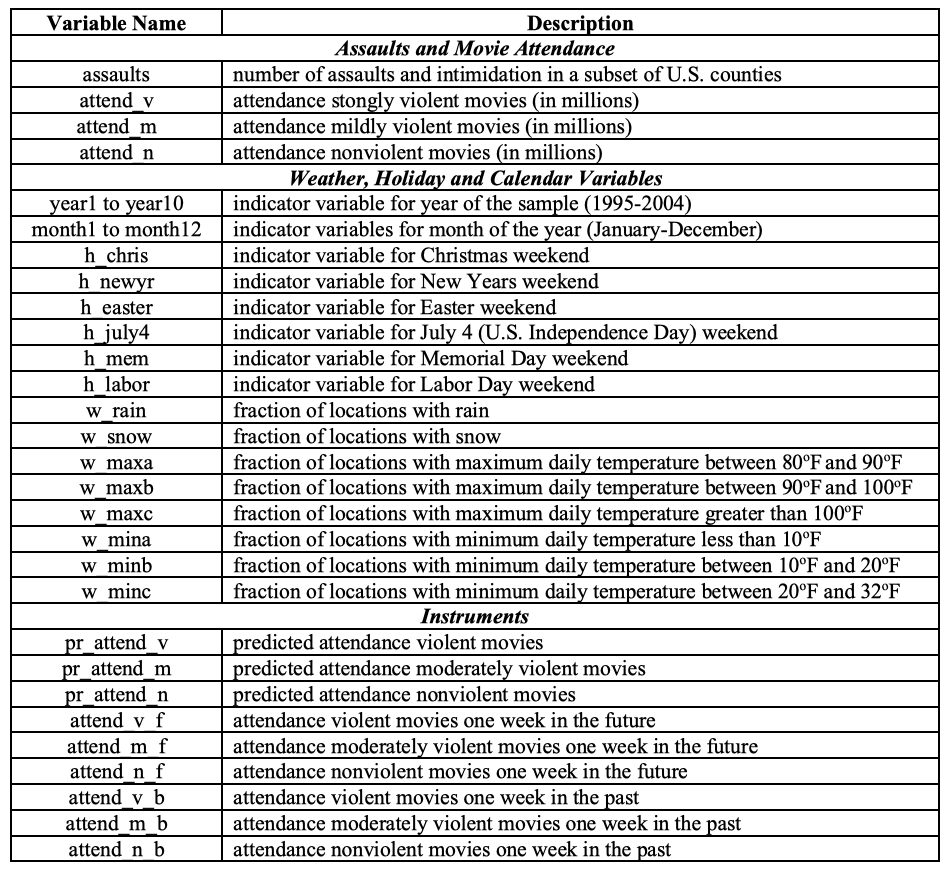
\includegraphics[width=0.6\textwidth]{Images/L4-1_1.png}

\end{frame}


%%
\begin{frame}[fragile]{EE12.2 a(i.)}

To detect whether there is time trend or not:
$$log(assaults) = \beta_0 + \psi_1 year + \psi_2 month + u$$

Or just simply graph a twoway plot with the time indicator.

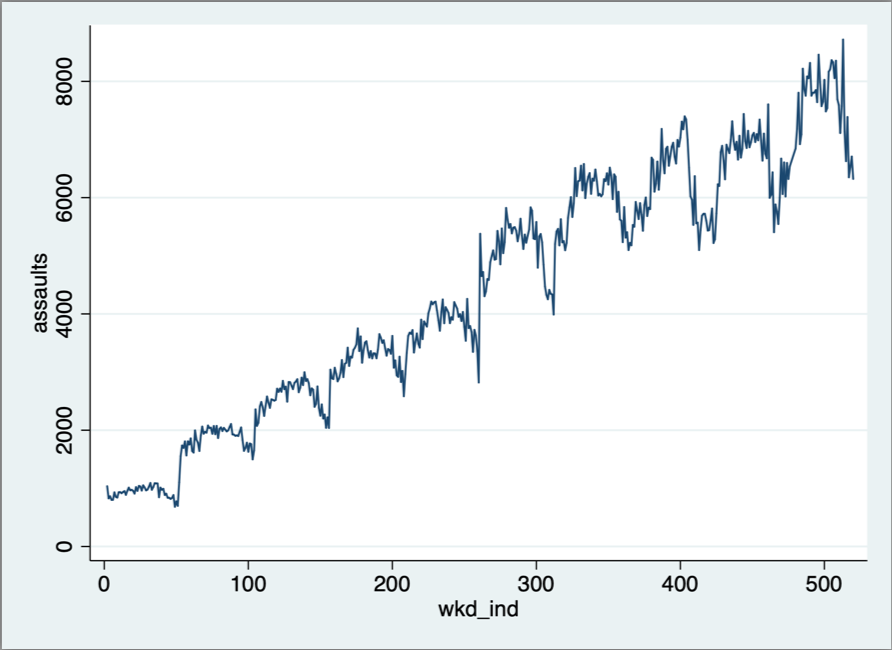
\includegraphics[width=0.8\textwidth]{Images/L4-1_2.png}

\end{frame}


%%
\begin{frame}[fragile]{EE12.2 a(ii.)}

To detect whether there is time trend or not:
$$attendance = \beta_0 + \phi_1 year + \phi_2 month+ \tilde{u}$$

Or just simply graph a twoway plot with the time indicator.

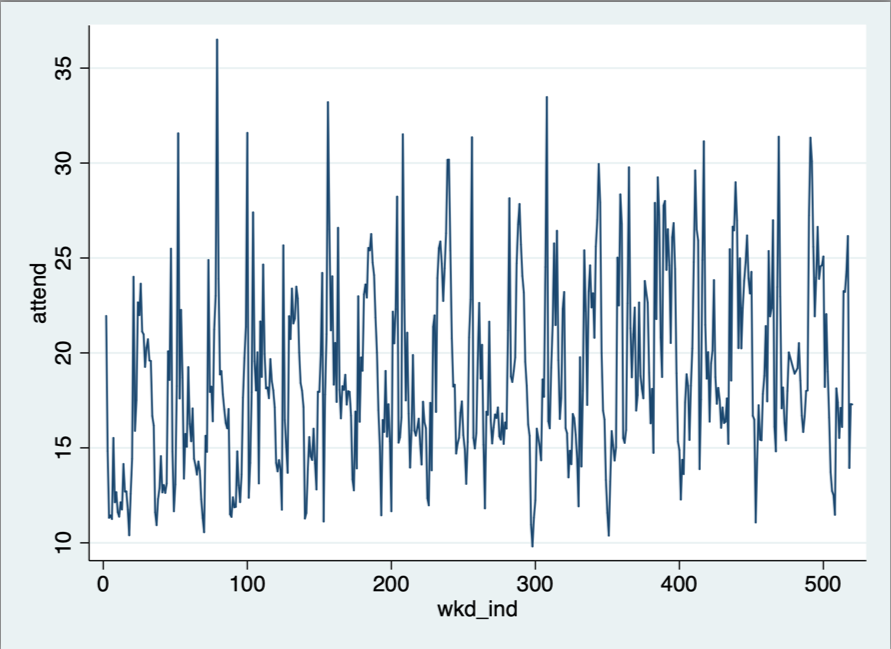
\includegraphics[width=0.8\textwidth]{Images/L4-1_3.png}

\end{frame}


%%
\begin{frame}[fragile]{EE12.2 b}

The original model is:
$$log(assaults) = \beta_0 + \beta_1 attend\textunderscore v +\beta_2 attend\textunderscore m+\beta_3 attend\textunderscore n+ \phi Time+\psi Controls$$

And the variables of interest are \texttt{attend\textunderscore v, attend\textunderscore m, attend\textunderscore n}

Till now, we do not say the variables of interest are exog. or endog.

\end{frame}


%%
\begin{frame}[fragile]{EE12.2 b(iii.)}

The original model is:
$$log(assaults) = \beta_0 + \beta_1 attend\textunderscore v +\beta_2 attend\textunderscore m+\beta_3 attend\textunderscore n+ \phi Time+\psi Controls$$

What we want to know is the change in the dependent variable: $\Delta assaults$.

Let's start from: 
$$\Delta log(assaults) = {\beta_1} \Delta attend\textunderscore v + {\beta_2} \Delta attend\textunderscore m+{\beta_3} \Delta attend\textunderscore n$$

Then,

$$\Delta \widehat{log(assaults)} = \hat{\beta_1} \Delta attend\textunderscore v + \hat{\beta_2} \Delta attend\textunderscore m+\hat{\beta_3} \Delta attend\textunderscore n$$

With the description in the questions:
$$\Delta \widehat{log(assaults)} = 6\hat{\beta_1} - 2 \hat{\beta_2}-\hat{\beta_3}$$

\end{frame}


%%
\begin{frame}[fragile]{EE12.2 b(iii.)}

$$\Delta \widehat{log(assaults)} = 6\hat{\beta_1} - 2 \hat{\beta_2}-\hat{\beta_3}$$

And we can easily calculate the estimate: $\Delta \widehat{log(assaults)} = -.01063206$

That is: $\Delta \widehat{assaults} \approx e^{-.01063206}$

\end{frame}


%%
\begin{frame}[fragile]{EE12.2 b(iii.) conti.}

Given $\Delta \widehat{log(assaults)} = 6\hat{\beta_1} - 2 \hat{\beta_2}-\hat{\beta_3}$

To obtain $se(\Delta \widehat{log(assaults)}) = se(6\hat{\beta_1} - 2 \hat{\beta_2}-\hat{\beta_3})$,

we need to apply approaches in section 7.3.

We may simplify the model by:

$$y =\beta_0 + \beta_1 v+\beta_2 m + \beta_3 n + u$$
Now let's focus on $\beta_1 v+\beta_2 m + \beta_3 n$ only.

Our goal is to have a explanatory variable which has a coefficient equals to the above number.

\end{frame}


%%
\begin{frame}[fragile]{EE12.2 b(iii.) conti.}

Simplified model:

$$y =\beta_0 + \beta_1 v+\beta_2 m + \beta_3 n + u$$

$$y = \beta_1 v+\beta_2 m + \beta_3 n -6\beta_1 n+2\beta_2 n + 6\beta_1 n-2\beta_2 n +u$$

$$y = \beta_1 (v+6n)+\beta_2 (m-2n) + (\beta_3-6\beta_1+2\beta_2) n +u$$

Now we can simply use OLS to obtain the s.e.
\end{frame}

%%
\begin{frame}[fragile]{EE12.2 c}

Now we want to use IVs.

Notations:

$Y: dependent variable$


$X: possibly endog. expanatory variables$

$W: exog. expanatory variables$

$Z: instrument variables$


Recall the 2SLS:

\begin{itemize}
    \item Regress X on Z, W
    \item Obtain $\hat{X}$
    \item Regress Y on $\hat{X}, W$
    \item Obtain the coef. of $\hat{X}$
\end{itemize}

\end{frame}


%%
\begin{frame}[fragile]{EE12.2 c}

Denote

$Y: log(assaults)$

$X: attend\textunderscore v, attend\textunderscore m, attend\textunderscore n$

$W: Time, Holiday, Weather$

$Z: pr\textunderscore attend\textunderscore v, pr\textunderscore attend\textunderscore m, pr\textunderscore attend\textunderscore n$

which are predictions based on historical attendance patterns.

THINK: Why are these variable instruments?

We'll demonstrate the manual 2SLS approach first.

\end{frame}


%%
\begin{frame}[fragile]{EE12.2 c}

We may simply use \texttt{ivreg} or \texttt{ivregress}

The format would be:

\texttt{ivreg Y (X=Z) W, r}

or:

\texttt{ivregress 2sls Y (X=Z) W, r}

\texttt{ivregress gmm Y (X=Z) W, r}

\end{frame}


%%
\begin{frame}[fragile]{EE12.2 d}

Now change the IVs:
$$Z: attend\textunderscore v\textunderscore f, attend\textunderscore m\textunderscore f, attend\textunderscore n\textunderscore f,
\\attend\textunderscore v\textunderscore b, attend\textunderscore m\textunderscore b, attend\textunderscore n\textunderscore b$$

which are the lagged terms and the future terms.

\end{frame}


%%
\begin{frame}[fragile]{EE12.2 e}

For Overidentifying Restriction Test, we first apply J-Test in textbook p.449, then we'll demonstrate a simple and more general command in Stata.

Note that the model now is: 

$Y = \beta X + \gamma W +u$  This is (12.12) in p.438

Denote the residuals obtained in the above regression as $\hat{u}_{2SLS}$.

Then we regress $\hat{u}_{2SLS}$ on $Z, W$, that is:
$$\hat{u}_{2SLS} = \delta Z + \tilde{\gamma} W + e$$
\end{frame}

%%
\begin{frame}[fragile]{EE12.2 e}
And we can obtain the J-statistic from $J=mF$ where

$m = \text{the number of instruments}$

$F = \text{the joint test statistic of } \delta=0}$

$k = \text{the number of exog. variables}$

Under homosk., $J \sim \chi^2(m-k)$
\end{frame}


%%
\begin{frame}[fragile]{EE12.2 e}

An easy command is:

\begin{verbatim}
ivregress Y (X=Z) W, r
estat overid
\end{verbatim}

will give you the test statistic under robust variance covariance estimator.

\end{frame}






    \section{Quasi Experiment EE13.1}




%%
\begin{frame}[fragile]{EE12.2}

我們直接從課本的Empirical Exercise 13.1來複習如何用Stata實作quasi-experimental analysis,並做出解釋。

\end{frame}

%%
\begin{frame}[fragile]{EE13.1 Questions}
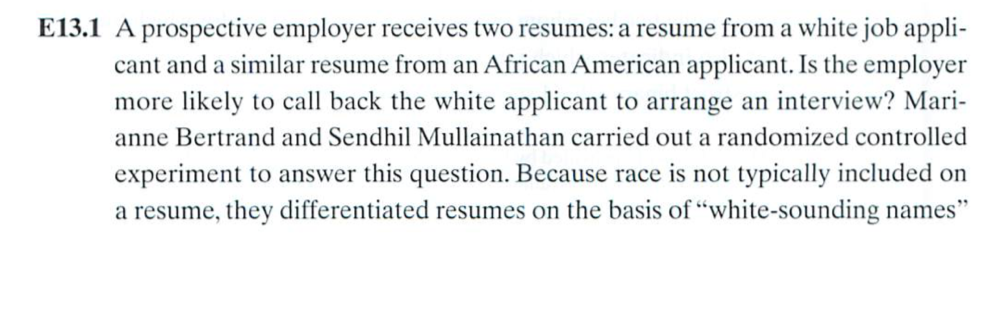
\includegraphics[width=1\textwidth]{Images/EE13-1_1.png}
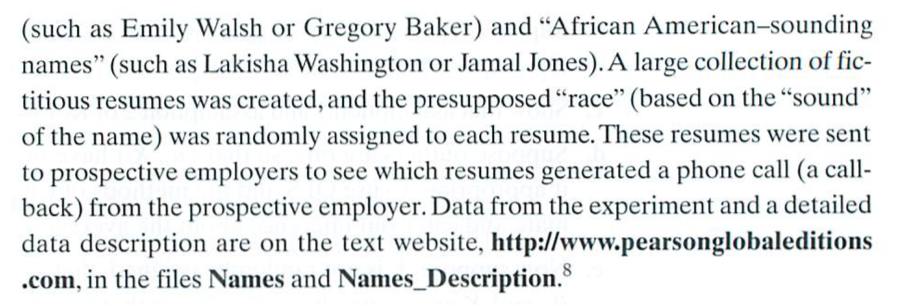
\includegraphics[width=1\textwidth]{Images/EE13-1_2.png}
\end{frame}
%%
\begin{frame}[fragile]{EE13.1 Questions}
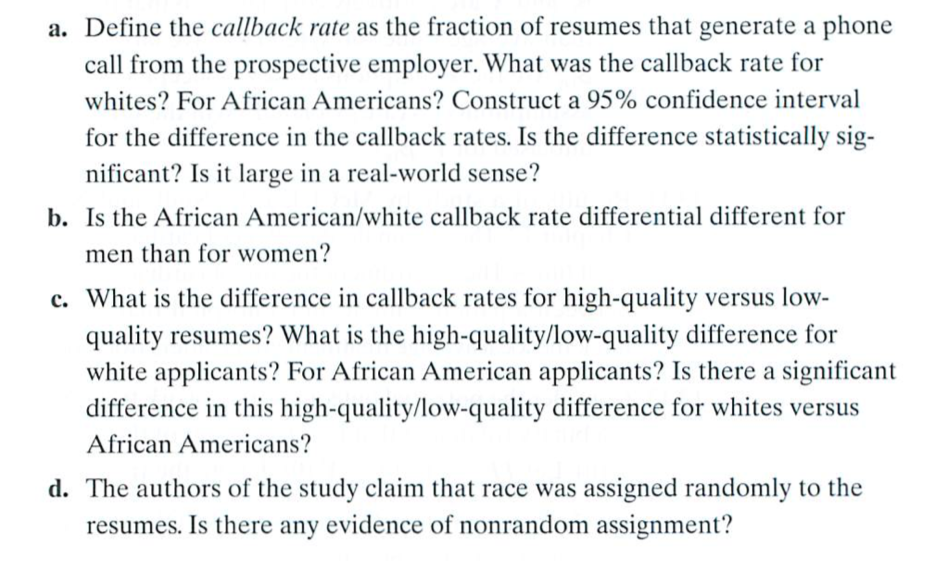
\includegraphics[width=1\textwidth]{Images/EE13-1_3.png}
\end{frame}



%%
\begin{frame}[fragile]{EE13.1 Data Descrptions}

Names Data

\begin{enumerate}
    \item Observations: 4870 resumes
    \item Time Period : 2001
\end{enumerate}
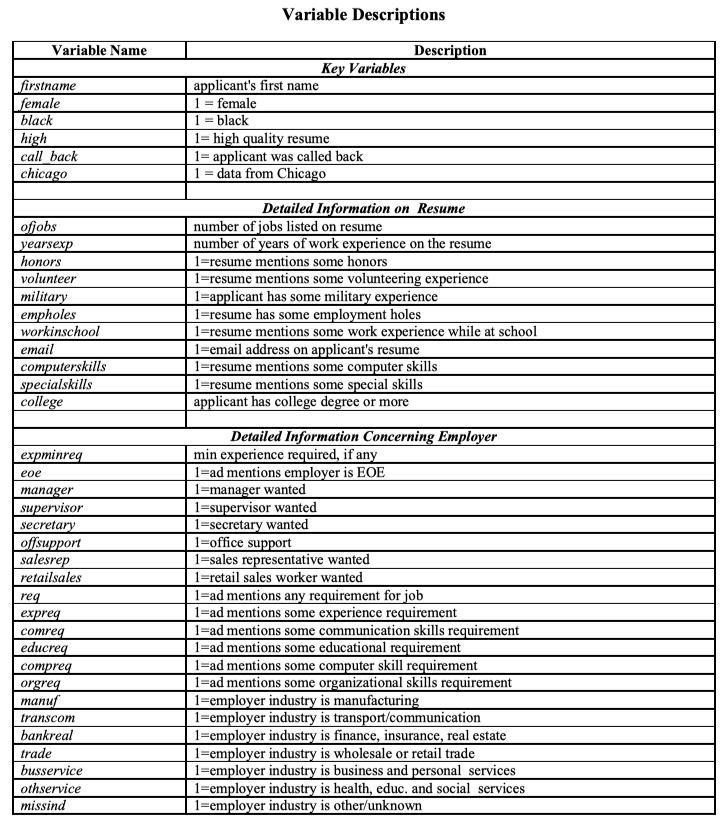
\includegraphics[width=0.5\textwidth]{Images/EE13-1_4.png}

\end{frame}


%%
\begin{frame}[fragile]{EE13.1 a}

The command:

\texttt{mean callback} 

gives us the fraction of resumes that generate a phone call from prospective employer.

The expression:

\texttt{ci mean callback} 

gives us the same result.
\end{frame}


%%
\begin{frame}[fragile]{EE13.1 a}

For whites, simply add a condition:

\texttt{ci mean callback if black==0}

For blacks:

\texttt{ci mean callback if black==1}

\end{frame}


%大刮號binary寫法:https://blog.csdn.net/miao0967020148/article/details/78712811
%
\begin{frame}[fragile]{EE13.1 a conti.}

To understand how Stata gives us the 95\% C.I., recall the point estimator in the previous semester.

Let $$ y_i=\left\{
\begin{aligned}
1 & , \text{if receive phone call}\\
0 & , \text{o.w.}\\
\end{aligned}
\right.$$

Clearly, $y_i$ follows $Bernoulli(p)$ where $p$ is the unknown fraction of resumes that generate a phone call from prospective employer.

Naturally, we would like to use $\bar{y} = \frac{1}{n}\sum_{i=1}^n y_i$ to estimate $p$. Where $n=4870$.

We need to know $se(\bar{y})$ in order to build up a interval estimator.

\end{frame}


%
\begin{frame}[fragile]{EE13.1 a conti.}

Now, our concern would be: What is the sampling distribution of $\bar{y}$?

Given $$y_i \stackrel{i.i.d.}{\sim} Bernoulli(p)$$

then $$\sum_{i=1}^n y_i \sim Binomial(n, p)$$

which can be approximated by normal distribution $$\sum_{i=1}^n y_i \stackrel{a}{\sim} N(np, np(1-p))$$ as $n \rightarrow \infty$. And let $X = \frac{1}{n} \sum_{i=1}^n y_i$, then $$X \sim N(p, \frac{p(1-p)}{n})$$

That is, $se(\bar{y})$ can be calculated easily from the approximated normal distribution.
\end{frame}


%
\begin{frame}[fragile]{EE13.1 a conti.}

With the normal quantile $Z_{0.05} = -1.96$, we know the interval estimator for $p$ is:


[$ \bar{y}-1.96\times se(\bar{y}), \bar{y}+1.96 \times se(\bar{y}) $]


And we know $se(\bar{y}) \approx (0.0804928(1-.0804928)/4870)^{\frac{1}{2}} = 0.003898446728$

Which is nearly the \texttt{Std. Err.} calculated by Stata.

After that, we may construct the C.I. under every given quantile.

\end{frame}


%
\begin{frame}[fragile]{EE13.1 a conti.}

Some may know that the command:

\texttt{ci proportion callback}

gives us a very similar result, and wonder the difference between the two.

Actually, you may see the text "Binomial Exact" in the latter command.

That is, Stata calculate the exact sampling distribution from "categories" we're interested in, instead of using the approximated normal distribution.

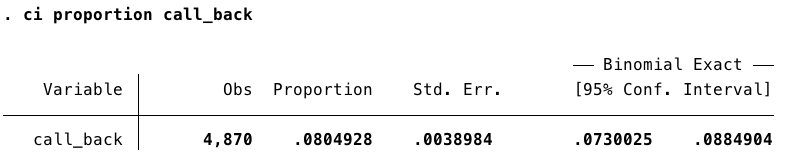
\includegraphics[width=1\textwidth]{Images/L4-2_1.png}

\end{frame}


%
\begin{frame}[fragile]{EE13.1 a conti.}
Also, if the variable is binary, and it is valued at 1 and 0, then the two command will yield the same result as the number of observations is large.

And the option \texttt{proportion} is designed for category variables. You may notice that there are Binomial distribution, Trinomial distribution, and Multinomial distribution.

For example, 
$$(X, Y) \sim Trinomial (n, p_1, p_2)$$
$$f_{XY}(x, y) = \frac{n!}{x!y!(n-x-y)!}p_1^x p_2^y (1-p_1-p_2)^{n-x-y}$$

\end{frame}





%
\begin{frame}[fragile]{EE13.1 b}

Given the model:
$$call\_back = \beta_0 + \beta_1 black + \beta_2 female + \beta_3 black\time female + u$$

If $black=0$ \& $female=0$, then the effect is $\beta_0$

If $black=1$ \& $female=0$, then the effect is $\beta_0+\beta_1$

If $black=0$ \& $female=1$, then the effect is $\beta_0+\beta_2$

If $black=1$ \& $female=1$, then the effect is $\beta_0+\beta_1+\beta_2+\beta_3$

\end{frame}


%
\begin{frame}[fragile]{EE13.1 c}

Given the model:
$$call\_back = \beta_0 + \beta_1 black + \beta_2 high + \beta_3 black\time high + u$$

If $black=0$ \& $high=0$, then the effect is $\beta_0$

If $black=1$ \& $high=0$, then the effect is $\beta_0+\beta_1$

If $black=0$ \& $high=1$, then the effect is $\beta_0+\beta_2$

If $black=1$ \& $high=1$, then the effect is $\beta_0+\beta_1+\beta_2+\beta_3$

\end{frame}




%%
\begin{frame}[fragile]{EE13.1 Table}
\begin{table}[htbp]
\small

\begin{tabular}{lccc} \hline
 & (1) & (2) & (3) \\
VARIABLES & a & b & c \\ \hline
 &  &  &  \\
black & -0.0320*** & -0.0304* & -0.0231** \\
 & (0.00778) & (0.0155) & (0.0106) \\
female &  & 0.0102 &  \\
 &  & (0.0137) &  \\
blackFemale &  & -0.00224 &  \\
 &  & (0.0179) &  \\
high &  &  & 0.0229* \\
 &  &  & (0.0120) \\
blackHigh &  &  & -0.0178 \\
 &  &  & (0.0156) \\
Constant & 0.0965*** & 0.0887*** & 0.0850*** \\
 & (0.00599) & (0.0119) & (0.00801) \\
 &  &  &  \\
Observations & 4,870 & 4,870 & 4,870 \\
 R-squared & 0.003 & 0.004 & 0.004 \\ \hline
\multicolumn{4}{c}{ Robust standard errors in parentheses} \\
\multicolumn{4}{c}{ *** p$<$0.01, ** p$<$0.05, * p$<$0.1} \\
\end{tabular}


\end{table}
\end{frame}

    
    %\input{chapters/03-Reshape.tex}
    
    

\section{Stata Homework 5 Announcement}


%
\begin{frame}[fragile]{HW}
    \begin{enumerate}
        \item Textbook Empirical Exercise 12.1 (a.)-(f.)
        \item Notice that (g.) is not included.
    \end{enumerate}

\end{frame}

%
\begin{frame}[fragile]{HW格式要求}
    \begin{enumerate}
        \item Upload only one pdf file.
        \item All formula should be expressed in LaTeX format.
        \item Deadline is 6/2 Tue. 14:10
    \end{enumerate}


\end{frame}

%
\begin{frame}[fragile]{Example Answers}
    Check Stata handout.
\end{frame}



%
\begin{frame}[fragile]{EE12.1 Questions}
    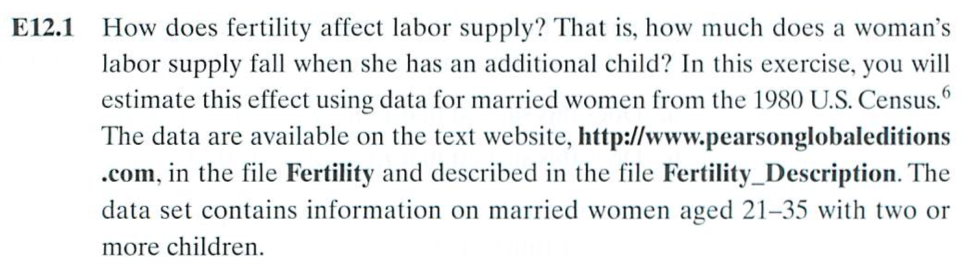
\includegraphics[width=1\textwidth]{Images/EE12-1_1.png}
\end{frame}

%
\begin{frame}[fragile]{EE12.1 Questions}
    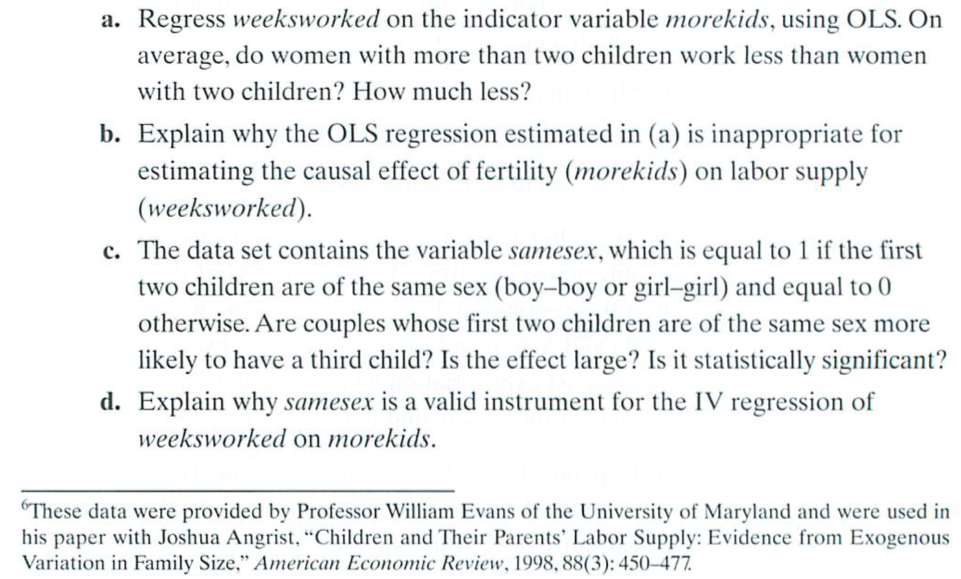
\includegraphics[width=1\textwidth]{Images/EE12-1_2.png}
    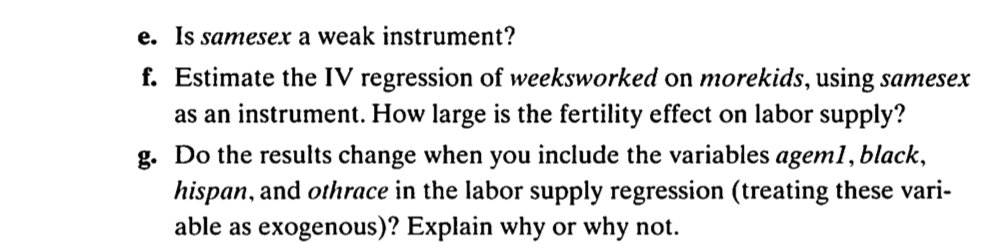
\includegraphics[width=1\textwidth]{Images/EE12-1_3.png}
\end{frame}


%\begin{frame}{Q and A}
%        \centering
%            \Huge\bfseries
%        \textcolor{orange}{Any question is welcomed!}
%    \end{frame}

%    \begin{frame}{Bye!}
%        \centering
%            \Huge\bfseries
%        \textcolor{orange}{Thank you}
%    \end{frame}



\end{document}










 %   \section*{References} 
 %   \nocite{Li_Norman2018} \nocite{Kamenica_Gentzkow2011} \nocite{Sunstein2005} \nocite{Gentzkow_Kamenica2017}
 %   \nocite{Gentzkow_Kamenica2017a}
 %       \begin{frame}[allowframebreaks]{References}
 %          \printbibliography
 %       \end{frame}